\documentclass[11pt]{beamer}
\usetheme{Warsaw}
\usepackage[utf8]{inputenc}
\usepackage[russian]{babel}
\usepackage[T2A]{fontenc}
\usepackage{amsmath}
\usepackage{amsfonts}
\usepackage{amssymb}
\usepackage{graphicx}
\author{Журавская, Камалбеков, Козловцев \\ 517 группа}
\title{Speaker recognition}
%\setbeamercovered{transparent} 
%\setbeamertemplate{navigation symbols}{} 
%\logo{} 
\institute{Московский Государственный Университет имени М.В.Ломоносова \\
Факультет вычислительной математики и кибернетики \\
Кафедра математических методов прогнозирования }


\date{24 июня 2019 г.} 


\setbeamertemplate{navigation symbols}{}

\begin{document}

\begin{frame}
\titlepage
\end{frame}

\begin{frame}
\frametitle{Постановка задачи}
\textbf{Дано:} образцы голосов $N$ спикеров; \\ 
Обучающая и тестовая выборки; \\
У каждого спикера уникальный $id$.\\
\vspace{2em}
\textbf{Найти:} для каждого образца в тестовой выборке либо подобрать $id$ спикера, либо определить, что таких $id$ в обучающей выборке нет.
\end{frame}

\begin{frame}
\frametitle{Наивный алгоритм}
\begin{itemize}
\item Признаки: mfcc из второго задания! 
\item Разделим пространство признаков на кластеры: K-Means!
\item Найдем порог принадлежности кластеру: если расстояние от объекта до всех центров кластеризации больше порога, то считаем, что спикер новый, т.е. его не было в обучающей выборке.
\end{itemize}
\vspace{1em}
Детали: Количество признаков 24. Количество кластеров $4N$*. \\
Проблемы: плохая разделимость, низкая скорость работы
\vfill
*\href{https://pdfs.semanticscholar.org/32c4/db25607bd52a6d0aeb5498ec9c8d564e6d2e.pdf?_ga=2.263177676.1944660485.1561369829-1562048709.1560510651}{Speaker identification using mel frequency
cepstral coefficients}
\end{frame}

\begin{frame}
\frametitle{VGGist}
\begin{itemize}
\item Данные: \href{http://www.robots.ox.ac.uk/~vgg/data/voxceleb/}{VoxCeleb} аудио + видео!
\item Предобработка: ....
\item Сеть: \href{https://github.com/tensorflow/models/tree/master/research/audioset/vggish}{VGGish на GitHub}
\end{itemize}
Проблемы: tf -> torch, свою сеть обучать долго: используем предобученную!\\
\vfill
Итог: точность $\approx 20\%$ на 100 спикерах с наибольшим количеством образцов голоса.
\end{frame}


\begin{frame}
\frametitle{Мы не сдаёмся}
\href{https://medium.com/analytics-vidhya/building-a-speaker-identification-system-from-scratch-with-deep-learning-f4c4aa558a56}{Building a Speaker Identification System from Scratch with Deep Learning}
\begin{itemize}
\item Данные: \href{http://www.openslr.org/12/}{LibriSpeech}
\item Архитектура:
\end{itemize}
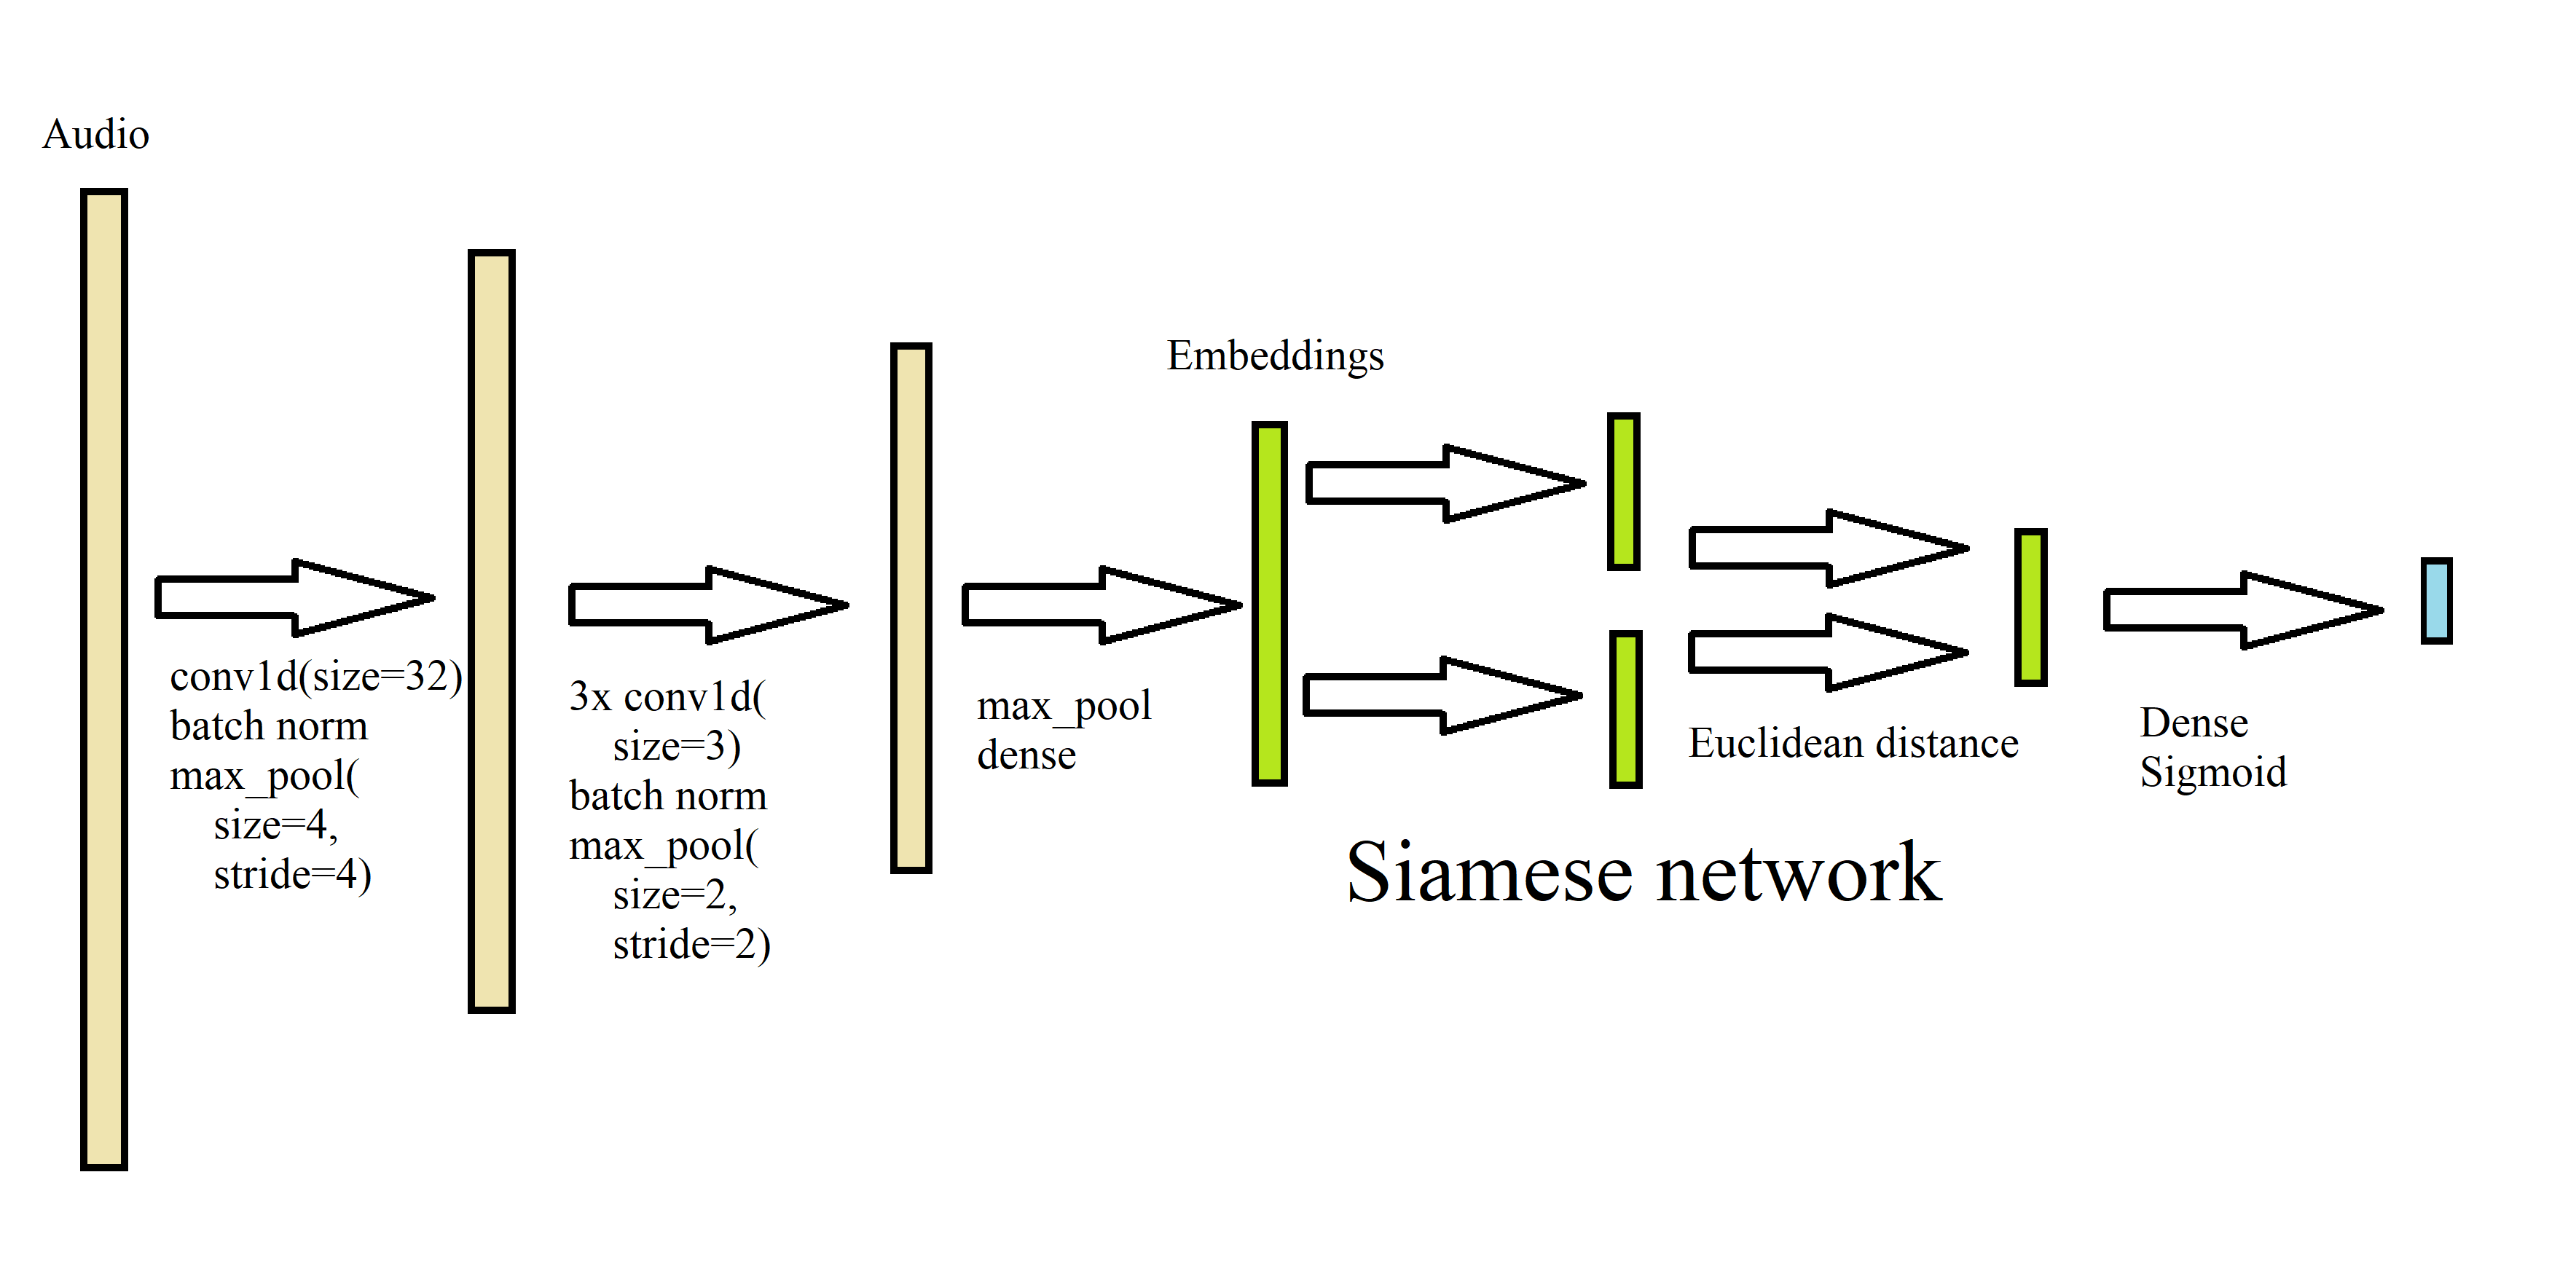
\includegraphics[width = \linewidth]{siamese.png}
\end{frame}

\begin{frame}
\frametitle{Эксперименты}

Датасет: LibriSpeech
\begin{itemize}
\item train-clean-100 -- 100 часов <<чистой>> английской речи, 250 различных людей;
\item train-clean-360 -- 360 часов <<чистой>> английской речи;
\item test-clean -- 40 различных пользователей.
\end{itemize}

Идея: будем использовать кодировщик из предобученной <<сиамской>> сети для преобразования признакового пространства.

\end{frame}

\begin{frame}
\frametitle{Эксперименты. Эмбеддинги}

\begin{figure}[htp]
\centering
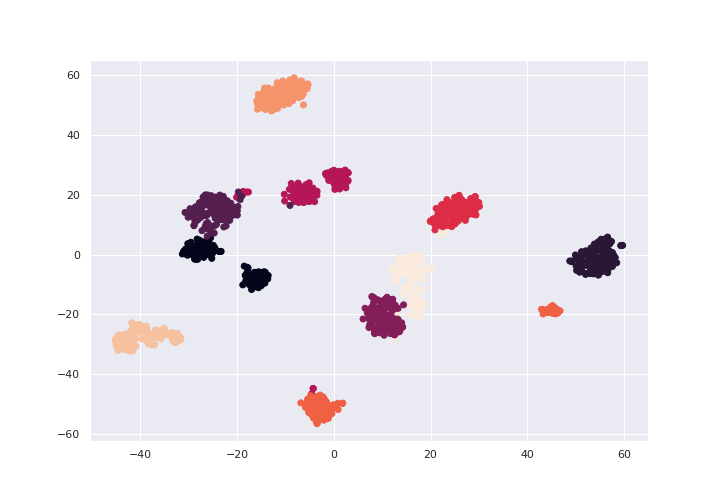
\includegraphics[scale=0.40]{test_emb.png}
\caption{Эмбеддинги тестовых записей}
\label{}
\end{figure}

\end{frame}

\begin{frame}
\frametitle{Эксперименты. K-shot learning}

Как точно мы можем идентифицировать человека, если до этого наблюдали не более $k$ элементов каждого класса? Классификация -- KNN.

\begin{figure}[htp]
\centering
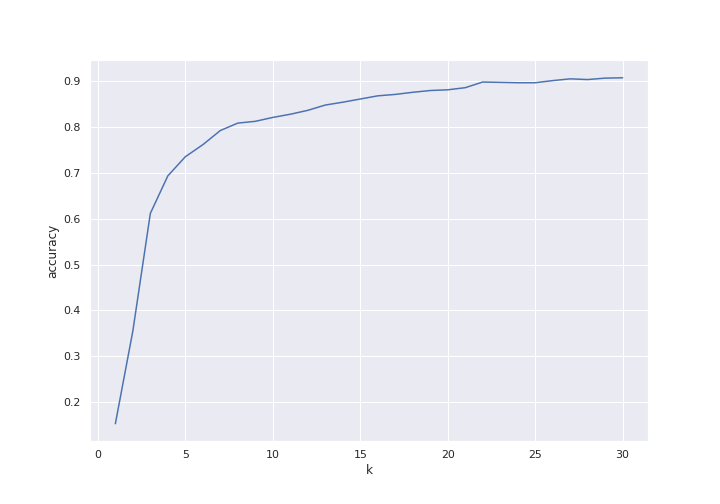
\includegraphics[scale=0.32]{k-shot.png}
\caption{Влияние $k$ на качество модели}
\label{}
\end{figure}

\end{frame}

\begin{frame}
\frametitle{Эксперименты. Transfer Learning}

\begin{table}[h!]
\begin{center}

\begin{tabular}{|c|c|c|c|}
\hline
	Алгоритм & Accuracy \\
\hline
	KNN на эмбеддингах & 94.4\% \\
\hline
	KNN на усреднённых эмбеддингах & 83.3\% \\
\hline
	Случайный лес & 93.1\% \\
\hline
	Градиентный бустинг & 91.2\% \\
\hline
\end{tabular}
\caption{Сравнение моделей}
\end{center}
\end{table}
\end{frame}


\begin{frame}
\frametitle{Заключение}
Мы изучили существующие методы решения задачи распознавания спикера. Мы попробовали несколько методов распознавания на нескольких наборах данных. Получили опыт использования предобученных нейронных сетей. \\
\vspace{1em}
Наилучший результат получен с использованием siamese networks, точность классификации на наборе данных LibriSpeech $ 94.4 \%$!\\
\vfill
\textbf{Вклад участников:}
\begin{tabular}{ll}
Саша & идея, наивный алгоритм, презентация \\
Костя & сеть: выбор архитектуры, перенос весов \\
Тимур & данные: предобработка и эксперименты
\end{tabular}
\end{frame}

\end{document}

